

In David helps Goliath, the authors find the generation no longer updates for the last 40\% of the inference time. They incorporate an early-stop strategy: halting the small model from generation based on empirically determined time range: \textit{t = 0.4T}, the pipeline reduces the total number of denoising steps by 40\% without sacrificing output quality. \cite{han_david_2024} 

Building on ideas from autoregressive speculative decoding, Speculative Diffusion Decoding uses a fast DLLM as a draft generator and an AR model as the verifier. The diffusion draft draws $k$ tokens in parallel and the AR target then confirms or corrects them, yielding substantial speedups even without fine-tuning the diffusion draft \cite{christopher_speculative_2025}. This two-stage process highlights how parallel sampling can be combined with selective sequential verification to accelerate decoding.

Self-conditioned discrete diffusion processes can match autoregressive latency through parallel sampling. In their work on \textbf{SEDD}, Lou \emph{et al.} demonstrate that around 100 denoising steps suffice to match AR inference time, and by removing KV-cache dependencies, throughput can increase by 4–6× \cite{lou_discrete_2024}. This result highlights the potential of batch parallelism and cache-free sampling in reducing the speed gap between diffusion and autoregressive models.

Task-specific optimizations also yield notable gains. The \textbf{Discrete Diffusion Language Model for Efficient Text Summarization} employs tailored noise schedules and reduced-step denoising to outperform both AR and continuous-diffusion baselines on wall-clock decoding time \cite{dat_discrete_2025}. By focusing computation on the most informative tokens, the efficiency of summarization is greatly enhanced.

Reparameterization of discrete diffusion versus continuous dynamics has a significant impact on convergence speed. Zheng \emph{et al.} analyze how continuous diffusion over token embeddings converges slowly—meaningful tokens only emerge after hundreds or thousands of iterations—while reparameterized discrete diffusion achieves coherent text generation in tens of steps, explaining much of the observed speed disparity \cite{zheng_reparameterized_2024}.

In Energy-Based Diffusion Language Models, a pretrained AR model serves as an energy function within the diffusion sampler. By applying importance sampling on late timesteps, required denoising steps can be reduced while maintaining AR-level generation quality under the same latency budget \cite{xu_energy-based_2025}. This approach illustrates how energy-based rejection sampling can accelerate diffusion inference.

Finally, \textbf{Your Absorbing Discrete Diffusion} removes time-conditioning in its Markov kernel to enable KV-style caching of intermediate predictions, further speeding up sampling compared to standard absorbing diffusion formulations \cite{ou_your_2025}. This caching mechanism highlights how architectural modifications can alleviate the overhead of iterative denoising.

\begin{figure*}[ht]
    \centering
    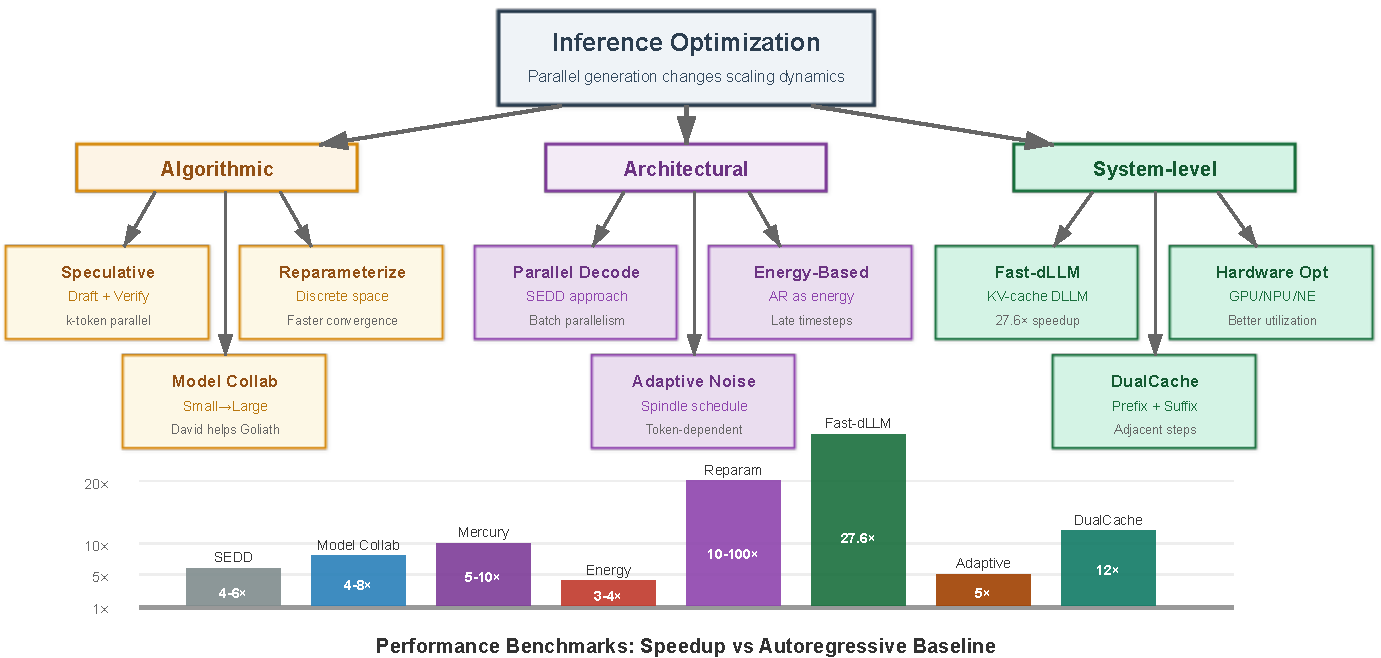
\includegraphics[width=1.0\textwidth]{figs/8_inference_speed.pdf}
    \caption{DLLM Inference Speed Optimization Techniques}
    \label{fig:dllm_inference_speed}
\end{figure*}

% \bibliographystyle{plain}
% \bibliography{DLLM}